\chapter{Einleitung} 

Durch längere Lagerung und thermische Belastung kann in Honig Hydroxymethylfurfural (HMF) in größerer Konzentration entstehen. HMF steht im Verdacht krebserregend zu sein. Zudem ist ein niedriger Gehalt an HMF ein Indikator für die Frische und Naturbelassenheit von Honig.
\begin{figure}[htbp]
	\centering
		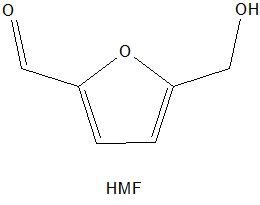
\includegraphics[width=0.5\textwidth]{../Bilder/HMF.jpg}
	\caption{Hydroxymethylfurfural}
	\label{fig:HMF}
\end{figure}
\newline
Eine Möglichkeit HMF in Honig zu bestimmen, ist die photometrische Methode nach WINKLER. Mittels einer Farbreaktion wird ein rot erscheinender Farbstoff erzeugt, der anschließend quantifiziert wird. Zur  Bestimmung des HMF-Gehalts wird zunächst die Methode, wie in dem Buch Lebensmittelanalytik~\cite{Lebensmittelanalytik} beschrieben, nachgestellt. Da in der zur Verfügung stehenden Methode lediglich ein Festfaktor zur Quantifizierung angegeben ist, wird zusätzlich eine Kalibrierreihe mit mehreren Messwerten durchgeführt. Des Weiteren wird die Methode auf Reproduzierbarkeit überprüft. Zur Ermittlung des Massenanteils an HMF werden mehrere Arten der Quantifizierung verwendet. Diese sind zum einen die Berechnung über den angegebenen Festfaktor, die Verwendung der erstellten Kalibriergeraden, sowie über Aufstockung einer Probe mit anschließender Standardadditionsberechnung. Es werden acht verschiedene Honige, ein Zuckerrübensirup und eine Invertzuckermischung, die bei Raumtemperatur aufbewahrt wurden, vermessen. Außerdem werden sechs der Honige für zehn Tage bei $60^\circ$ C gelagert und ein Anstieg des HMF-Gehalts nachgewiesen. Die Handhabung der Proben ist durch ihre Viskosität erschwert. Da der Honig viele verschiedene, zum Teil unlösliche Bestandteile enthält, wird diese Matrix vor der Bestimmung entfernt. Die verwendeten Chemikalien erfordern wegen ihrer gefährlichen Eigenschaften eine besonders sorgfältige Handhabung. Ihre Haltbarkeit ist auch bei korrekter Lagerung begrenzt. Der bei der Derivatisierung entstandene Farbstoff ist nicht stabil und zerfällt nach wenigen Minuten, deshalb muss jede Lösung zeitlich exakt vermessen werden.~\cite{Winkler}